% ==============================================================================
% TCC - Nome do Aluno
% Capítulo 3 - Especificação de Requisitos
% ==============================================================================
\chapter{Especificação de Requisitos e Análise do SCAP}
\label{sec-requisitos}

Este capítulo apresenta uma descrição de escopo referente ao SCAP (Sistema de Controle de Afastamento de Professores), assim como o modelo de casos de uso e o diagrama de classes que foi levantado anteriormente por~\citeonline{duarte-pg14} e posteriormente analisado por~\citeonline{prado-pg15}. 

\section{Descrição do Escopo}
\label{sec-requisitos-descricao-escopo}

O SCAP surgiu com o objetivo de auxiliar o Departamento de Informática (DI) da UFES no controle e no registro de solicitações de afastamento do seus professores, para que eles possam participar de eventos que acontecem no Brasil e no exterior. Essas solicitações de afastamento necessitam passar por uma série de avaliações para que sejam aprovadas. Elas são avaliadas pelos professores do DI e dependendo do caso, também devem ser avaliadas pelo Centro Tecnológico (CT) e pela Pró-Reitoria de Pesquisa e Pós-Graduação (PRPPG). Nestes casos, somente após receber a aprovação de todas as instâncias, o afastamento é publicado no Diário Oficial da União e o professor recebe a autorização para participar do evento.     

A Câmara Departamental (composta pelos representantes discentes e pelos funcionários do departamento) fica responsável por avaliar e aprovar as solicitações de afastamento para eventos no Brasil. O chefe do departamento (cargo ocupado por um professor do DI por meio de um mandato temporário) recebe a solicitação de afastamento pelo email e após dez dias, se nenhum membro da Câmara Departamental for contra ao pedido, o afastamento é aprovado. Assim, para eventos nacionais, o processo permanece dentro do DI.

Para pedidos de afastamento referente a eventos internacionais, um professor (sem parentesco com o solicitante) é escolhido para se tornar relator do pedido. Assim que o relator manda o parecer, o pedido passa por avaliação para aprovação como no caso descrito com eventos que são realizados no Brasil. Para que o pedido seja publicado no Diário Oficial da União, ele deve receber a aprovação do CT e da PRPPG. Entretanto, o SCAP não possui uma integração com os processos do CT e da PRPPG, fazendo com que o controle das tramitações permaneça dentro do DI, restringindo o escopo do sistema.

Com o intuito de automatizar as tramitações das solicitações de afastamento, o SCAP auxilia os professores e secretários do DI, facilitando o processo desde a criação até a aprovação e armazenamento. Com o envio de e-mails automáticos para os envolvidos e com a utilização de formulários para a criação dos documentos necessários, o sistema pode ser considerado fundamental para esse processo.      

\section{Modelo de Casos de Uso}
\label{sec-requisitos-modelo-casos-uso}

Após o levantamento de requisitos e da definição do escopo, os atores identificados no sistema SCAP são apresentados na Tabela~\ref{tabela-atores-scap}.  

\begin{table}[h]
	\centering	
	\vspace{0.5cm}
	\footnotesize
	\caption{Atores do SCAP~\cite{duarte-pg14}.}	
	\label{tabela-atores-scap}
	\begin{tabular}{|p{5.0cm}|p{9.0cm}|}  \hline 
 		
 		\rowcolor[rgb]{0.8,0.8,0.8} \textbf{Ator} & \textbf{Descrição} \\\hline 
		
		\textbf{Professor} & Professores efetivos do DI/UFES. \\\hline
		
		\textbf{Chefe do Departamento} & Professores do DI/UFES que estão realizando a função administrativa de chefe e subchefe do departamento. \\\hline
		
		\textbf{Secretário} & Secretário do DI/UFES. \\\hline
		
	\end{tabular}
\end{table}

A parte administrativa do sistema fica por conta dos \textbf{secretários}. Eles possuem a responsabilidade de realizar o cadastro dos mandatos dos chefes do departamento, realizar o cadastro dos professores e dos seus respectivos parentescos. Quando surgem pareceres de fora do DI e quando os pedidos de afastamento são finalizados, os \textbf{secretários} também ficam responsáveis pelo controle dessas tarefas.

O SCAP fornece algumas funcionalidades para os \textbf{professores}. Eles podem realizar o cadastro das solicitações de afastamento e realizar uma manifestação contra o afastamento de outro professor, caso ainda esteja dentro do prazo. Além disso, o \textbf{professor} fica responsável por recomendar a aprovação ou não de um afastamento no exterior, caso ele seja adicionado como relator do mesmo. 

Se um \textbf{professor} se tornar \textbf{chefe do departamento} por meio de um mandato, ele deve realizar o encaminhamento de solicitações aos relatores que farão o deferimento de pareceres com relação aos afastamentos internacionais.

O diagrama de casos de uso do SCAP pode ser visualizado por meio da Figura~\ref{fig-requisitos-casos-uso}. Uma pequena descrição dos casos de uso será apresentada nos próximos parágrafos e uma versão mais completa dessa descrição pode ser encontrada em~\cite{duarte-pg14,prado-pg15}.
     
\begin{figure}[h]
	\centering
	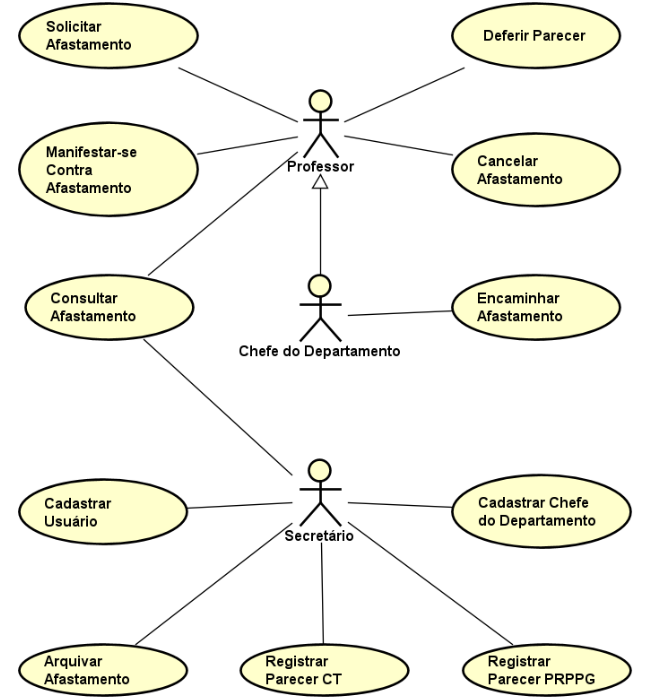
\includegraphics[scale=0.5]{figuras/fig-requisitos-casos-uso} 
	\caption{Diagrama de Casos de Uso do SCAP.}
	\label{fig-requisitos-casos-uso}
\end{figure}

No sistema, um professor realiza o cadastro de um pedido de afastamento por meio do caso de uso \textbf{Solicitar Afastamento}, fornecendo todos os dados que são necessários para realizar a tramitação. Um professor pode cancelar uma solicitação de afastamento utilizando o caso de uso \textbf{Cancelar Afastamento}, realizando a alteração do status para cancelado.

Após escolher um relator para um pedido de afastamento internacional, o Chefe do Departamento pode executar o caso de uso \textbf{Encaminhar Afastamento}. Quando um professor que se tornou relator por meio da indicação do Chefe do Departamento realizar o cadastro do seu parecer sobre o afastamento, o caso de uso \textbf{Deferir Parecer} pode ser utilizado.

Um professor, um chefe de departamento ou um secretário podem utilizar o caso de uso \textbf{Consultar Afastamento} assim que necessitarem obter informações sobre uma solicitação de afastamento. Se um professor for contra a um pedido de afastamento, o caso de uso \textbf{Manifestar-se Contra Afastamento} pode ser utilizado e após o motivo ser cadastrado, uma reunião é agendada para decidir a aprovação ou reprovação da solicitação.

Um secretário realiza o cadastramento de novos professores ou secretários por meio do caso de uso \textbf{Cadastrar Usuário}, onde são informados todos os dados necessários. Um secretário também utiliza o caso de uso \textbf{Cadastrar Chefe do Departamento} para especificar o período do mandato do novo chefe do departamento.
  
Quando existe uma solicitação de afastamento internacional, um secretário realiza o cadastro do parecer do Centro Tecnológico e da Pró-Reitoria de Pesquisa e Pós-Graduação por meio dos casos de uso \textbf{Registrar Parecer CT} e \textbf{Registrar Parecer PRPPG}.

O caso de uso \textbf{Arquivar Afastamento} é executado após a tramitação de uma solicitação de afastamento ser realizada, fazendo com que um secretário realize a alteração do status para ``Arquivado''.   

\section{Análise do SCAP}
\label{sec-requisitos-analise-scap}

O diagrama de classes do SCAP pode ser visualizado por meio da Figura~\ref{fig-requisitos-diagrama-classes}. As instâncias das classes são especificadas de acordo com o comportamento exercido pelos objetos que seguem as especificações das classes. 

\begin{figure}[h]
	\centering
	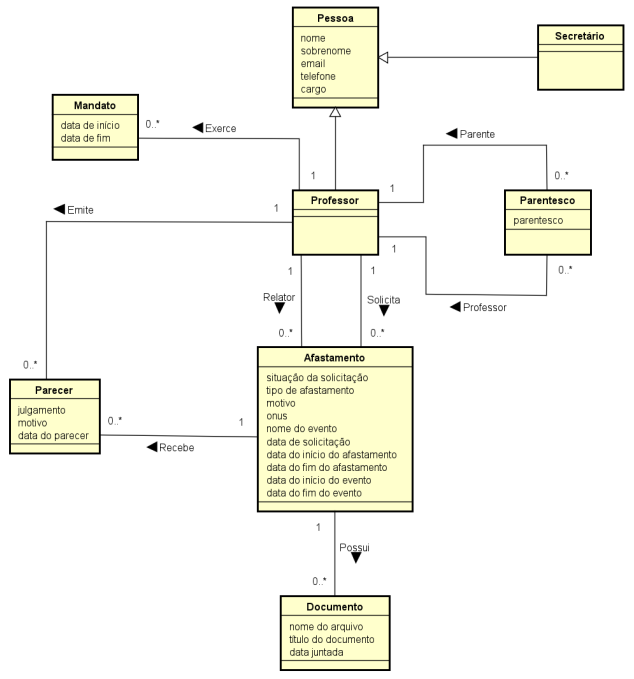
\includegraphics[scale=0.7]{figuras/fig-requisitos-diagrama-classes} 
	\caption{Diagrama de Classes do SCAP.}
	\label{fig-requisitos-diagrama-classes}
\end{figure}

Herdando todos os atributos da classe \textbf{Pessoa}, os professores são representados pela classe \textbf{Professor} e os secretários são representados pela classe \textbf{Secretário}. Os professores podem possuir relações de parentesco, seja ela matrimonial ou sanguínea. Essas relações são representadas pela classe \textbf{Parentesco}. Um professor pode ocupar o cargo de chefe ou subchefe do departamento, sendo que o tempo de permanência no cargo é representado pela classe \textbf{Mandato}.

Os pedidos de afastamento solicitados por professores são representados pela classe \textbf{Afastamento}. Nela se encontram todas as informações necessárias para realizar as tramitações. Esta classe pode conter documentos que são visualizados por meio da classe \textbf{Documento}. Quando um pedido de afastamento se trata de um evento internacional, a relação \textbf{Relator} deve ser utilizada informando o professor que foi indicado para isso.

A classe \textbf{Parecer} é utilizada quando um professor efetua a emissão de um parecer com relação a um afastamento. Um professor pode se tornar relator e criar pareceres de vários afastamentos diferentes. 

Restrições de integridade do sistema foram identificadas por \citeonline{duarte-pg14} e, após concluir a implementação de uma nova versão, \citeonline{prado-pg15} verificou que existia a necessidade de adicionar novas restrições. As restrições de integridade do SCAP que foram atualizadas estão descritas a seguir:
 
\begin{itemize}

	\item Um professor não pode ser relator de um afastamento solicitado por um parente;
	
	\item O secretário do departamento não pode abrir uma solicitação de afastamento;
	
	\item Não pode haver mais de dois professores (chefe e subchefe de departamento) exercendo um mandato ao mesmo tempo;
	
	\item A data de início de um mandato de professor não pode ser posterior a data de fim do mesmo mandato;
	
	\item A data de início de um afastamento não pode ser posterior a data de fim do mesmo afastamento;
	
	\item Um professor não pode ser solicitado para dar um parecer sobre sua própria solicitação de afastamento. 
   
\end{itemize} 
